Examine the data on paper-quality measurements in Table 1.2 for marginal and multivariate normality.


Paper is manufactured
in continuous sheets several feet wide.Because of the orientation of fibers
within the paper, it has a different strength when measured in the direction produced
by the machine than when measured across, or at right angles to, the machine
direction. Table 1.2 shows the measured values of

First, as mentioned on page 20, observations that are from old paper 16--21, 34, and 38--41 were deleted. Also, observation 25, which is a massive outlier was deleted.

For ($x_{1}$), we're using the measuring the paper density in grams/centimeter and have 29 valid observations. The simulated 0.01, 0.05, and 0.10 level critical correlation coefficient test values for a sample size of 29 are, 0.9473, 0.9637, and 0.9703, respectively. The Q-Q correlation coefficient using the raw data was 0.9838. This value is greater than all three critical values, so the data would be considered normally distributed at all three levels. If we left in the 12 observations deleted, this would absolutely not be the case.

We don't really need to transform the data, but just to see how much better it can get, the Box-Cox power transformation max was 4.3988, so $x_{2}^{\prime} = x_{2}^{4.3988}$. The Q-Q correlation coefficient on the transformed data was 0.9804, so we do get some improvement. Below is the Q-Q plot for the raw data, which looks pretty good.

\begin{center}
    \begin{figure}[H]
        \centering
        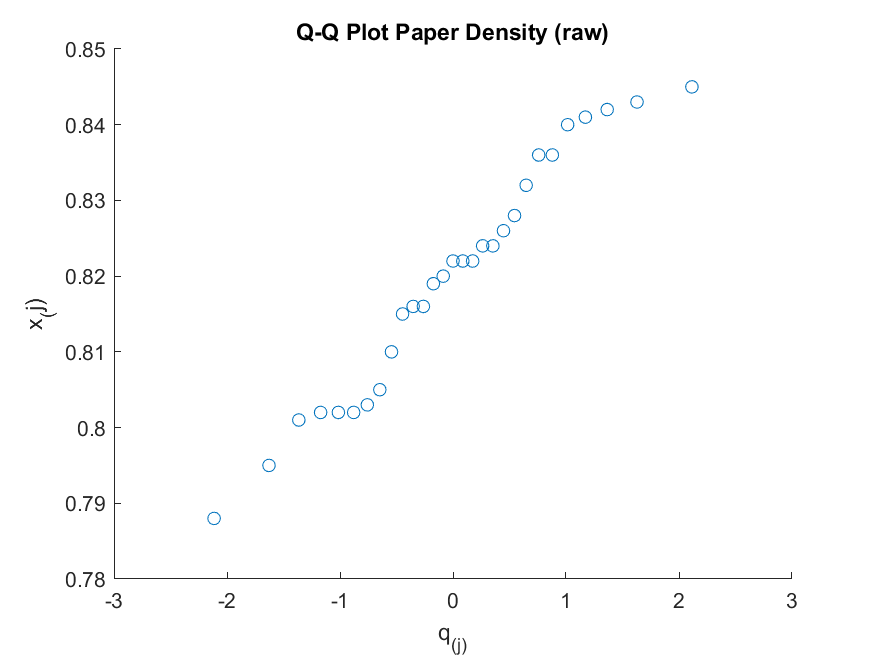
\includegraphics[scale=0.6]{./matlab/chapter-4/sol4.35.qq.1.png}
    \end{figure}
\end{center}

For ($x_{2}$), we're using the measuring the paper strength in the machine direction and have 29 valid observations. The simulated 0.01, 0.05, and 0.10 level critical correlation coefficient test values for a sample size of 29 are, 0.9473, 0.9637, and 0.9703, respectively. The Q-Q correlation coefficient using the raw data was 0.9911. This value is greater than all three critical values, so the data would be considered normally distributed at all three levels. If we left in the 12 observations deleted, this would absolutely not be the case.

We don't really need to transform the data, but just to see how much better it can get, the Box-Cox power transformation max was 1.7936, so $x_{2}^{\prime} = x_{2}^{1.7936}$. The Q-Q correlation coefficient on the transformed data was 0.9914, so we do get a very small improvement. Below is the Q-Q plot for the raw data, which looks pretty good.

\begin{center}
    \begin{figure}[H]
        \centering
        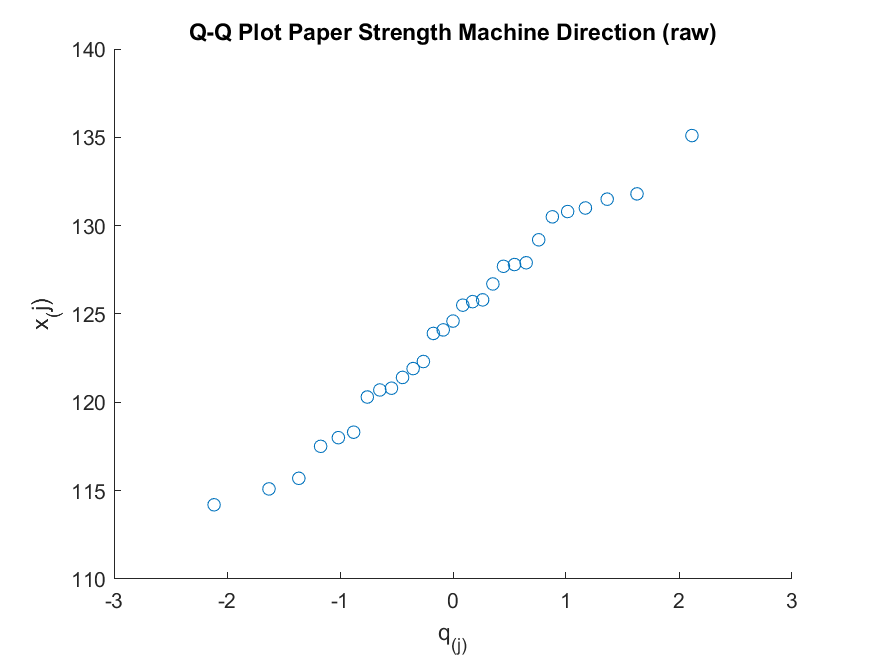
\includegraphics[scale=0.6]{./matlab/chapter-4/sol4.35.qq.2.png}
    \end{figure}
\end{center}

For ($x_{3}$), we're using the measuring the paper strength in the machine direction and have 29 valid observations. The simulated 0.01, 0.05, and 0.10 level critical correlation coefficient test values for a sample size of 29 are, 0.9473, 0.9637, and 0.9703, respectively. The Q-Q correlation coefficient using the raw data was 0.9789. This value is greater than all three critical values, so the data would be considered normally distributed at all three levels. If we left in the 12 observations deleted, this would absolutely not be the case.

We don't really need to transform the data, but just to see how much better it can get, the Box-Cox power transformation max was -2.4549, so $x_{2}^{\prime} = x_{2}^{-2.4549}$. The Q-Q correlation coefficient on the transformed data was 0.9810, so we do get a very small improvement. Below is the Q-Q plot for the raw data, which looks pretty good.

\begin{center}
    \begin{figure}[H]
        \centering
        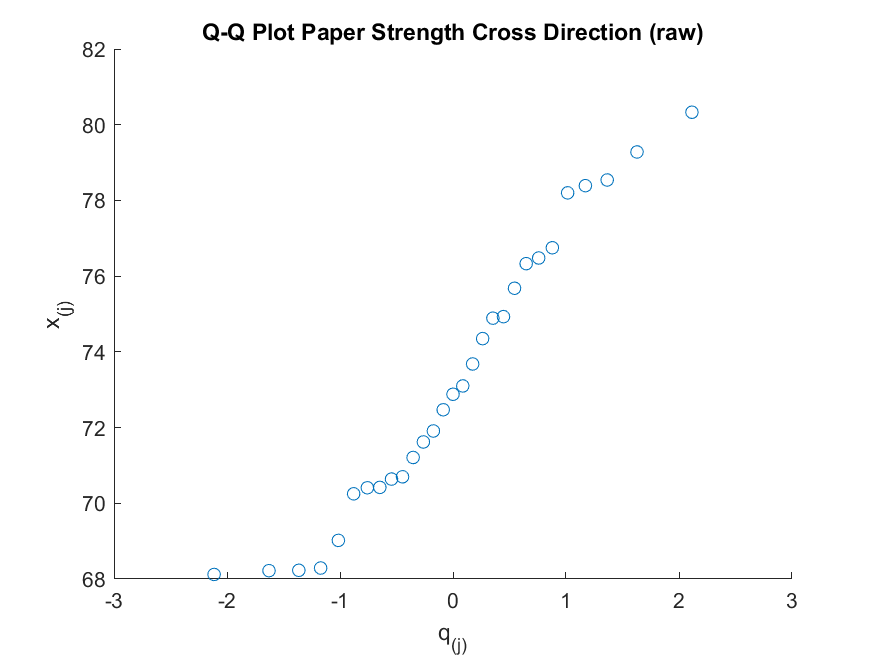
\includegraphics[scale=0.6]{./matlab/chapter-4/sol4.35.qq.3.png}
    \end{figure}
\end{center}


All of our variables are considered univariate normal, now to check the bivariate, we have ${3 \choose 2} = 3$ pairs of variables to evaluate for

\[
\left\{
    \begin{NiceArray}{cc}
        (x_{1}, x_{2}), & (x_{1}, x_{3}), \\
        (x_{2}, x_{3}) &                 \\
    \end{NiceArray}
\right\}
\]

\begin{table}[H]
    \caption*{Proportion less than $\chi_{2}^{2}(0.50) = 1.3863$}
    \centering
    \begin{tabular}{lc}
        \hline % chktex 44
        Variables & Raw Data \\
        \hline % chktex 44
        $(x_{1}, x_{2})$ & 0.3793 \\
        $(x_{1}, x_{3})$ & 0.3103 \\
        $(x_{2}, x_{3})$ & 0.4483 \\
        \hline % chktex 44
    \end{tabular}
\end{table}

We'd expect to see about 50\% of the data with distance values less than 1.3863, but all 3 variables have proportions are are fairly low. We only have 29 observations, so that might have something to do with it.